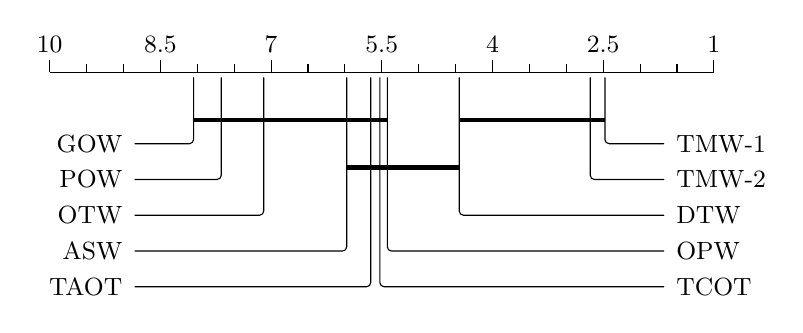
\begin{tikzpicture}[
  treatment line/.style={rounded corners=1.5pt, line cap=round, shorten >=1pt},
  treatment label/.style={font=\small},
  group line/.style={ultra thick},
]

\begin{axis}[
  clip={false},
  axis x line={center},
  axis y line={none},
  axis line style={-},
  xmin={1},
  ymax={0},
  scale only axis={true},
  width={\axisdefaultwidth},
  ticklabel style={anchor=south, yshift=1.3*\pgfkeysvalueof{/pgfplots/major tick length}, font=\small},
  every tick/.style={draw=black},
  major tick style={yshift=.5*\pgfkeysvalueof{/pgfplots/major tick length}},
  minor tick style={yshift=.5*\pgfkeysvalueof{/pgfplots/minor tick length}},
  title style={yshift=\baselineskip},
  xmax={10},
  ymin={-6.5},
  height={7\baselineskip},
  xtick={1.0,2.5,4.0,5.5,7.0,8.5,10.0},
  minor x tick num={2},
  x dir={reverse},
]

\draw[treatment line] ([yshift=-2pt] axis cs:2.475, 0) |- (axis cs:1.6416666666666666, -2.0)
  node[treatment label, anchor=west] {TMW-1};
\draw[treatment line] ([yshift=-2pt] axis cs:2.675, 0) |- (axis cs:1.6416666666666666, -3.0)
  node[treatment label, anchor=west] {TMW-2};
\draw[treatment line] ([yshift=-2pt] axis cs:4.45, 0) |- (axis cs:1.6416666666666666, -4.0)
  node[treatment label, anchor=west] {DTW};
\draw[treatment line] ([yshift=-2pt] axis cs:5.425, 0) |- (axis cs:1.6416666666666666, -5.0)
  node[treatment label, anchor=west] {OPW};
\draw[treatment line] ([yshift=-2pt] axis cs:5.525, 0) |- (axis cs:1.6416666666666666, -6.0)
  node[treatment label, anchor=west] {TCOT};
\draw[treatment line] ([yshift=-2pt] axis cs:5.65, 0) |- (axis cs:8.883333333333335, -6.0)
  node[treatment label, anchor=east] {TAOT};
\draw[treatment line] ([yshift=-2pt] axis cs:5.975, 0) |- (axis cs:8.883333333333335, -5.0)
  node[treatment label, anchor=east] {ASW};
\draw[treatment line] ([yshift=-2pt] axis cs:7.1, 0) |- (axis cs:8.883333333333335, -4.0)
  node[treatment label, anchor=east] {OTW};
\draw[treatment line] ([yshift=-2pt] axis cs:7.675, 0) |- (axis cs:8.883333333333335, -3.0)
  node[treatment label, anchor=east] {POW};
\draw[treatment line] ([yshift=-2pt] axis cs:8.05, 0) |- (axis cs:8.883333333333335, -2.0)
  node[treatment label, anchor=east] {GOW};
\draw[group line] (axis cs:4.45, -2.6666666666666665) -- (axis cs:5.975, -2.6666666666666665);
\draw[group line] (axis cs:2.475, -1.3333333333333333) -- (axis cs:4.45, -1.3333333333333333);
\draw[group line] (axis cs:5.425, -1.3333333333333333) -- (axis cs:8.05, -1.3333333333333333);

\end{axis}
\end{tikzpicture}